\documentclass[showpacs, oneside, onecolumn, prl, amsmath, amssymb, nofootinbib, superscriptaddress, notitlepage]{revtex4-1}


\usepackage{cases}
\usepackage{amsmath}
\usepackage{amssymb}
\usepackage{amsfonts}
\usepackage{amssymb}
\usepackage{dcolumn}
\usepackage{bm}
\usepackage{bbm}
\usepackage{graphicx}
\usepackage{xcolor}
\usepackage{array}
\usepackage{subfigure}
\usepackage{hyperref}
\usepackage{multirow}

%%%%%%%%%%%%%%%%%%%%%%%%%%%%%%%%%%%%%%%%%%%%%%%%%%%%%%%%%%%%%%%%%%%%%%%%%%%%%%%%%%%
\newcommand{\bra}[1]{\langle #1\vert}
\newcommand{\ket}[1]{\vert #1\rangle}
\newcommand{\nn}{\nonumber \\}
\newcommand{\lag}{\langle}
\newcommand{\rag}{\rangle}
\newcommand{\cN}{{\cal N}}
\newcommand{\cA}{{\cal A}}
\newcommand{\gsim}{\mathrel{\hbox{\rlap{\lower.55ex \hbox {$\sim$}}
                   \kern-.3em \raise.4ex \hbox{$>$}}}}
\newcommand{\lsim}{\mathrel{\hbox{\rlap{\lower.55ex \hbox {$\sim$}}
                   \kern-.3em \raise.4ex \hbox{$<$}}}}

\newcommand\be{\begin{equation}}
\newcommand\ba{\begin{align}}
\newcommand\bas{\begin{align*}}
\newcommand\bt{\begin{table}}
\newcommand\bts{\begin{table*}}
\newcommand\bfig{\begin{figure}}
\newcommand\bfs{\begin{figure*}}
\newcommand\ee{\end{equation}}
\newcommand\ea{\end{align}}
\newcommand\et{\end{table}}
\newcommand\ets{\end{table*}}
\newcommand\efig{\end{figure}}
\newcommand\efs{\end{figure*}}
\newcommand\sothat{$\ \ \Rightarrow\ \ $}


\newcommand\blue{\textcolor{blue}}
\newcommand\gray{\textcolor{gray}}
\newcommand\red{\textcolor{red}}




\hypersetup{colorlinks=true,
            breaklinks=true,
            pdfstartview=Fit,
            linkcolor=blue,
            citecolor=green,
            urlcolor=blue}

\bibliographystyle{apsrev4-1}




%%%%%%%%%%%%%%%%%%%%%%%%%%%%%%%%%%%%%%%%%%%%%%%%%%%%%%%%%%%%%%%%%%%%%%%%%%%%%%%%%%%
\begin{document}
	
\title{Phys 512 Problem Set 1}


\author{JIAO Hao}

\maketitle
%%%%%%%%%%%%%%%%%%%%%%%%%%%%%%%%%%%%%%%%%%%%%%%%%%%%%%%%%%%%%%%%%%%%%%%%%%%%%%%%%%%



%%%%%%%%%%%%%%%%%%%%%%%%%%%%%%%%%%%%%%%%%%%%%%%%%%%%%%%%%%%%%%%%%%%%%%%%%%%%%%%%
\section{Problem 1}

Here I set the function as "np.exp(x)". Integrate from 0 to 1 and the max error is 0.00001.

~

\textbf{The result of intgrator wrote inclass:}

- n= 5,	 	 delta x= 0.25

- n= 9,	 	 delta x= 0.125

- n= 17, 	 delta x= 0.0625

- n= 17, 	 delta x= 0.0625

- n= 9,		 delta x= 0.125

- n= 17, 	 delta x= 0.0625

- n= 17, 	 delta x= 0.0625

The integration in class of np.exp(x) from 0 to 1 is 1.7182819740518918 

~

\textbf{The result of my way:}

- n= 5, 	 delta x= 0.25

- n= 9, 	 delta x= 0.125

- n= 17, 	 delta x= 0.0625

The integration of np.exp(x) from 0 to 1 is 1.7182819740518918 

~

For N times recursive, the way in class calls the function $2^{N+1}-1$ times,while my way calls the function $N$ times. So I save $2^{N-1}-(N-1)$ times.

(PS, calculate the area1 and area2 is once.)

Besides, if the error is not uniform over the whole interval, the code used in class may need even more steps at the region with large error.


~~~~

%%%%%%%%%%%%%%%%%%%%%%%%%%%%%%%%%%%%%%%%%%%%%%%%%%%%%%%%%%%%%%%%%%%%%%%%%%%%%%%%
\section{Problem 2}

To reach the accuracy of $10^{-6}$, I need 7 terms of Chebyshev polynomial (shown in the toppenal of fig.\ref{2-2-1}).

\bfig
	\centering
	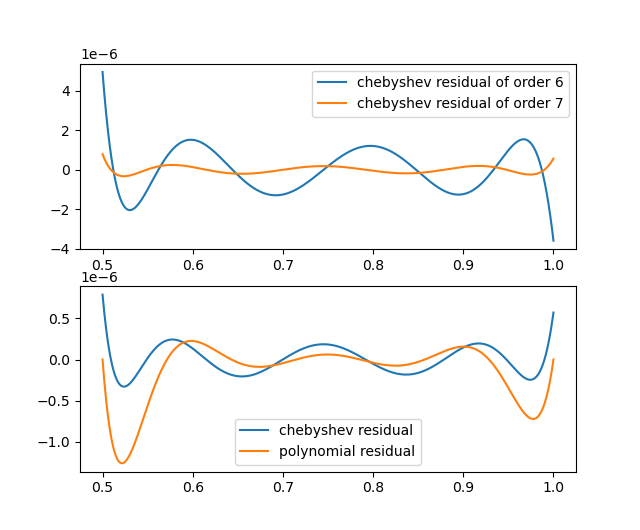
\includegraphics[scale=1]{2-2.png}
	\caption{Top penal: the residuals for Chebyshev polynomial of order 6 and 7. Bottom penal: compare the truncated Chebyshev and standard polynomial fits with the same order (7).}
	\label{2-2-1}
\efig

Plot the residuals for both the truncated Chebyshev and standard polynomial fits with the same order is show in the bottom penal of fig.\ref{2-2-1}.

~~~~

Compare the RMS error and max error of these two interpolation.

- For Chebyshev fit, the mean square error is 1.685e-07  and the maximum errors is  7.889e-07

- For same order Ploynomial fit, the mean square error is 3.480e-07  and the maximum errors is  1.260e-06

So the standard polynomial interpolation has both the higher RMS error and higher max error.


~~~~

~~~~

%%%%%%%%%%%%%%%%%%%%%%%%%%%%%%%%%%%%%%%%%%%%%%%%%%%%%%%%%%%%%%%%%%%%%%%%%%%%%%%%
\section{Problem 3}

\textbf{a) solve for the decay products of U238}

Which solver would you use for this problem?
I solve the ODE implicitly. Although it is less accurate, stiff solution is much faster than KR4 and this problem have to calculate over a very long period of time.

But there must be something wrong in this calculation: I solve the ODE in the interval $t=[0,10^{18}]s$ which is approximately 7 times of the halflife of U238. But in the end, the su of all y is much smaller than 1. I do not know why.


\textbf{b) Plot the ratio}

Plot the ratio of Pb206 to U238 as a function of time:

Assume that we can approximate the U238 decaying instantly to lead, so there only two states: U238 and Pb206 and the half-life is similar to the half-life of U238. I use both RK4 and stiff method here. Results are shown in fig.\ref{2-3-1}.

\bfig
	\centering
	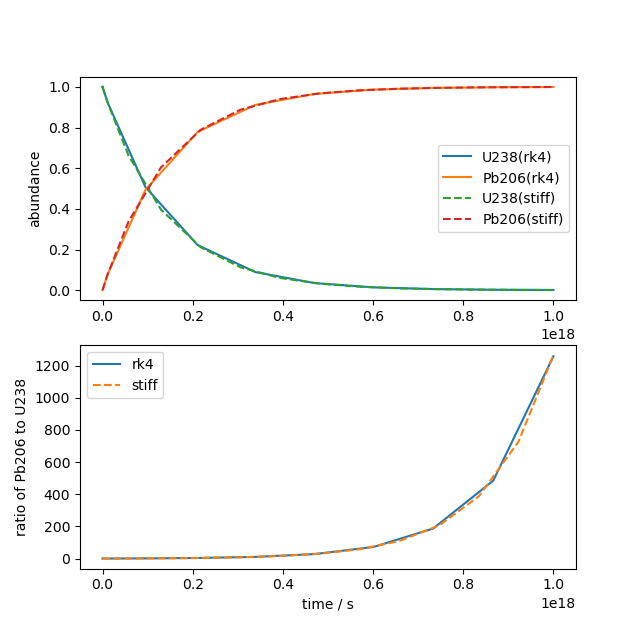
\includegraphics[scale=1]{2-3-1.png}
	\caption{Top penal: the abundance of U238 and Pb206 as a function of time. Bottom penal: the ratio of Pb206 to U238 as a function of time. I compare the two method RK4 and stiff here.}
	\label{2-3-1}
\efig


- it takes  0.0029916763305664062 s to solve the ODE with RK4

- it takes  0.09076476097106934 s to solve the ODE implicitly

The two method is similar to solve this ODE.

Does this make sense analytically?

Solving the ODE analytically, the abundance of U238 should decrease exponentially $\sim 2^{-t/\tau}$, so the abundance of Pb206 $\sim 1-2^{-t/\tau}$.

From this numerical solution, the abundance of U238 decay nearly exponentially (which is consistent with the physical picture of decay), and the abundance of Pb206 is approximate to 1-U238. So this result make sense.

~~~~

Plot the ratio of Thorium 230 to U234:

For simplification, I set the initial abundance of Th230 is 1. And the time interval is from 0 to 1e14 s.

 If we consider the decay of Th230 (which is faster than the decay of U234), the abundance of Th230 is approximate to 0 all over the time (fig.\ref{2-3-2}). If we ignore the decay of Th230, the evolution of abundance is similar to the case of U238 to Pb206 (fig.\ref{2-3-3}).

\bfig
	\centering
	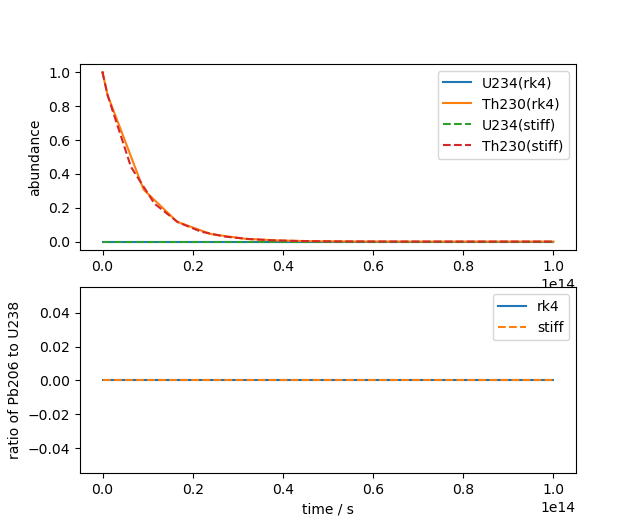
\includegraphics[scale=1]{2-3-2.png}
	\caption{Top penal: the abundance of U234 and Th230 as a function of time. Bottom penal: the ratio of Th230 to U234 as a function of time. I compare the two method RK4 and stiff here.}
	\label{2-3-2}
\efig

\bfig
	\centering
	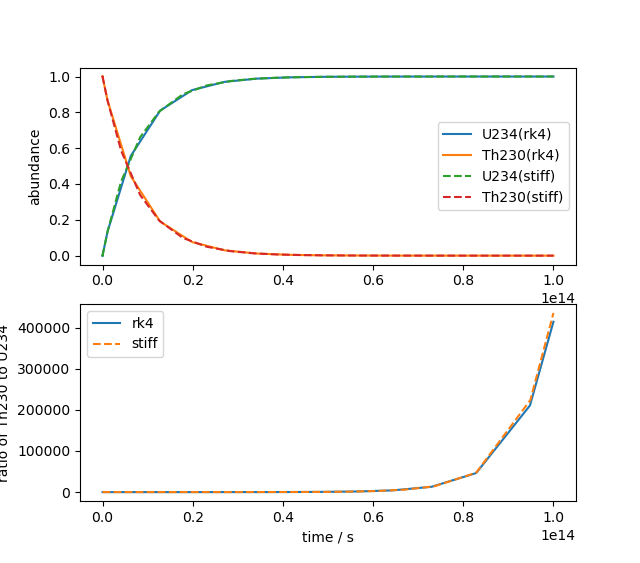
\includegraphics[scale=1]{2-3-3.png}
	\caption{Top penal: the abundance of U234 and Th230 as a function of time. Bottom penal: the ratio of Th230 to U234 as a function of time. I compare the two method RK4 and stiff here.}
	\label{2-3-3}
\efig




\end{document}